\documentclass[a4paper, 12pt]{article}
\usepackage[slovene]{babel}
\usepackage[utf8]{inputenc}
\usepackage{amsmath}
\usepackage{amssymb}
\usepackage{listings}
\usepackage{hyperref}
\usepackage{tikz}
\usetikzlibrary{positioning}
\usetikzlibrary{arrows}

\begin{document}
\title{Population dynamics in a food chain}
\author{Domen Mohorčič, Larsen Cundrič, Mustafa Grabus}
\maketitle

\section{Problem}
Modelirali bomo dinamiko populacij različnih vrst, odnosi med vrstami pa so predstavljeni
na naslednji sliki: \\
\begin{center}
	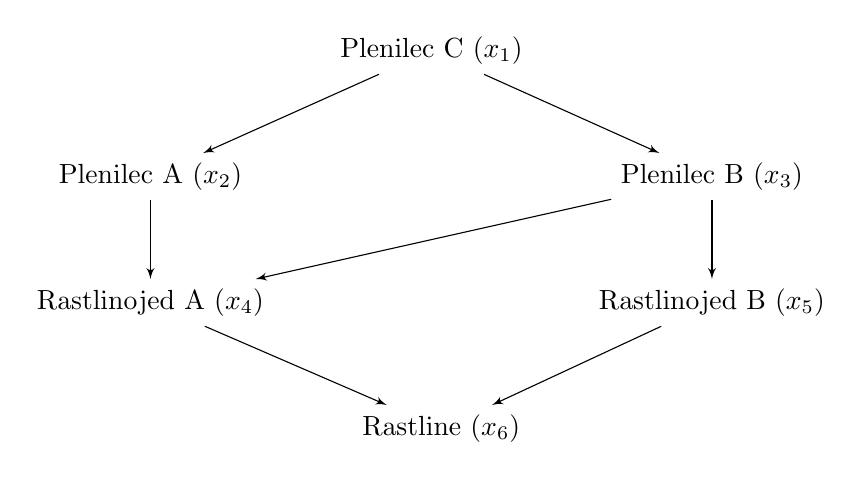
\begin{tikzpicture}
		\tikzset{edge/.style = {->,> = latex'}}
		\node (A) {Plenilec C ($ x_{1} $)};
		\node[below left=of A] (B) {Plenilec A ($ x_{2} $)};
		\node[below right=of A] (C) {Plenilec B ($ x_{3} $)};
		\node[below=of B] (D) {Rastlinojed A ($ x_{4} $)};
		\node[below=of C] (E) {Rastlinojed B ($ x_{5} $)};
		\node[below right=of D] (F) {Rastline ($ x_{6} $)};
		\draw[edge] (A) edge (B) edge (C);
		\draw[edge] (B) edge (D);
		\draw[edge] (C) edge (D) edge (E);
		\draw[edge] (D) edge (F);
		\draw[edge] (E) edge (F);
	\end{tikzpicture}
\end{center}
Puščice označujejo smer prehranjevanja (npr. Plenilec A se prehranjuje z Rastlinojedom A).
Z $ x_{i} $ označimo velikost posamezne populacije. Sprememba velikosti posamezne populacije
je tako odvisna od naravnega prirastka/smrtnosti, smrtnosti zaradi ulova in prirastka zaradi
prehranjevanja. Ulov in prehranjevanje sta odvisna od velikosti ustreznih drugih populacij,
naravni prirastek/smrtnost pa je odvisna samo od velikosti populacije. Dinamiko $ i $-te
populacije lahko opišemo tako:
\begin{equation}
	\dot x_{i} = x_{i}\cdot b_{i} + \sum_{i \not = j} a_{ij}\cdot x_{i}\cdot x_{j}
\end{equation}
kjer je $ x_{i} $ velikost $ i $-te populacije, $ b_{i} $ je koeficient naravnega prirastka/smrtnosti,
$ a_{ij}\cdot x_{i}\cdot x_{j} $ pa je sprememba $ i $-te populacije glede na interakcijo z $ j $-to populacijo.

\section{Reševanje}

\subsection{Naloga 1}
Sistem diferencialnih enačb za naš primer je naslednji:
\begin{align*}
	&\dot x_{1} = x_{1}\cdot(b_{1}+a_{12}\cdot x_{2}+a_{13}\cdot x_{3}) \\
	&\dot x_{2} = x_{2}\cdot(b_{2}+a_{21}\cdot x_{1}+a_{24}\cdot x_{4}) \\
	&\dot x_{3} = x_{3}\cdot(b_{3}+a_{31}\cdot x_{1}+a_{34}\cdot x_{4}+a_{35}\cdot x_{5}) \\
	&\dot x_{4} = x_{4}\cdot(b_{4}+a_{42}\cdot x_{2}+a_{43}\cdot x_{3}+a_{46}\cdot x_{6}) \\
	&\dot x_{5} = x_{5}\cdot(b_{5}+a_{53}\cdot x_{3}+a_{56}\cdot x_{6}) \\
	&\dot x_{6} = x_{6}\cdot(b_{6}+a_{64}\cdot x_{4}+a_{65}\cdot x_{5}) \\
\end{align*}
$ x_{i} $ predstavlja velikost i-te populacije, $ \dot x_{i} $ pa predstavlja spremembo
i-te populacije v odvisnosti od velikosti ostalih populacij. Velikosti posameznih vrst
bomo zapisali v vektor $ X = \left[x_{1}, x_{2}, x_{3}, x_{4}, x_{5}, x_{6}\right]^{T} $.
Sistem diferencialnih enačb pa bomo zapisali v vektor $ \dot X $:
\begin{equation}
	\dot X =
	\begin{bmatrix}
		\dot x_{1} \\
		\dot x_{2} \\
		\dot x_{3} \\
		\dot x_{4} \\
		\dot x_{5} \\
		\dot x_{6} \\
	\end{bmatrix}
	=
	\begin{bmatrix}
		x_{1}\cdot(b_{1}+a_{12}\cdot x_{2}+a_{13}\cdot x_{3}) \\
		x_{2}\cdot(b_{2}+a_{21}\cdot x_{1}+a_{24}\cdot x_{4}) \\
		x_{3}\cdot(b_{3}+a_{31}\cdot x_{1}+a_{34}\cdot x_{4}+a_{35}\cdot x_{5}) \\
		x_{4}\cdot(b_{4}+a_{42}\cdot x_{2}+a_{43}\cdot x_{3}+a_{46}\cdot x_{6}) \\
		x_{5}\cdot(b_{5}+a_{53}\cdot x_{3}+a_{56}\cdot x_{6}) \\
		x_{6}\cdot(b_{6}+a_{64}\cdot x_{4}+a_{65}\cdot x_{5}) \\
	\end{bmatrix}
\end{equation}
V vektorju $ b = \left[b_{1}, b_{2}, b_{3}, b_{4}, b_{5}, b_{6}\right]^{T} $ so koeficienti naravnega prirastka/smrtnosti,
ki je za rastline ($ x_{6} $) pozitiven, za vse ostale pa negativen. \\
Sistem enačb za dani primer lahko tako zapišemo kot
\begin{equation}
	\dot X = X*(b+A\cdot X)
\end{equation}
($ * $ predstavlja množenje po elementih),
kjer matrika $ A $ vsebuje koeficiente hranjenja in plenjenja $ a_{ij} $:
\begin{equation}
	A =
	\begin{bmatrix}
		0 & a_{12} & a_{13} & 0 & 0 & 0 \\
		a_{21} & 0 & 0 & a_{24} & 0 & 0 \\
		a_{31} & 0 & 0 & a_{34} & a_{35} & 0 \\
		0 & a_{42} & a_{43} & 0 & 0 & a_{46} \\
		0 & 0 & a_{53} & 0 & 0 & a_{56} \\
		0 & 0 & 0 & a_{64} & a_{65} & 0 \\
	\end{bmatrix}
\end{equation}
Koeficient $ a_{ij} $ predstavlja interakcijo vrste $ i $ in $ j $. Pozitivna vrednost pomeni, da se vrsta
$ i $ prehranjuje z vrsto $ j $, negativna pa ravno nasprotno. Vrsta s sabo nima take interakcije, zato
so elemeniti $ a_{i=j} = 0 $. Koeficienta $ a_{ij} $ in $ a_{ji} $ nista nujno nasprotna, saj lahko plenilska
vrsta poje več plena, kot pa ima koristi od tega. \\
Za začetek smo določili $ X = \left[\right]^{T} $,
$ b = \left[-0.2, -0.1, -0.1, -0.05, -0.05, 0.3\right]^{T} $ in $ A = ... $

\end{document}